\section{Praxisbeispiel DeepFaceLab}\label{sec:praxisbeispiel-dfl}
Im Folgenden wird der Workflow zum Erstellen von Video Deepfakes mit \gls{dfl} näher betrachtet.
Ziel dieses Kapitels ist das Tauschen zweier Gesichter in zwei Videos.
Für das Ersetzen in Echtzeit wird \gls{dflive} verwendet, dessen Workflow in einem anderen Kapitel (\ref{sec:deepfacelive}) beschrieben wird.

\subsection{Laborumgebung}\label{subsec:laborumgebung}
Alle Video-Deepfakes (\gls{dfl} und \gls{dflive}), wurden auf folgender Hardware erstellt.\\[0.5cm]
\begin{tabular}{rl}
    CPU:& \texttt{AMD Ryzen 5 2600X}\\
    RAM:& \texttt{16GB DDR4 3000MHz}\\
    GPU:& \texttt{NVIDIA RTX 2070 (8GB GDDR6 VRAM)}\\
    OS:& \texttt{Windows 11}
\end{tabular}\\[0.5cm]

Ziel des Deepfakes ist das Gesicht von \gls{rdj} auf Prof. Volker Knoblauch in diesem \href{https://www.youtube.com/watch?v=rksMPlRSbQU}{Video} zu swappen,
sodass die Hochschule Aalen amerikanische Prominente auf ihrem Youtube-Kanal zeigen kann.

\subsection{Programmstruktur}\label{subsec:programmstruktur}
Nach der Installation von \gls{dfl} finden sich im entsprechenden Ordner eine Vielzahl von \texttt{.bat}-Dateien, sowie ein \texttt{\_internal}- und \texttt{workspace}-Ordner.
Die \texttt{.bat}-Dateien führen die im \texttt{\_internal}-Ordner abgelegten Scripte mit den entsprechenden Parametern aus.
Es wäre also möglich auf diese Dateien zu verzichten und \gls{dfl} lediglich über eine Konsole auszuführen.
Alle Dateien, die während der Erstellung eines Deepfakes erstellt oder benötigt werden, werden im \texttt{workspace}-Ordner abgelegt.
Bei der Installation von \gls{dfl} werden Beispieldaten mitgeladen.\\

Immer wieder finden sich die Bezeichnungen \texttt{src} und \texttt{dst}.
Diese referenzieren in \gls{dfl}:
\begin{itemize}
    \item \textbf{src (Source):} Das Gesicht, bzw. das zugehörige Videomaterial, das über das Zielgesicht gelegt werden soll.
    \item \textbf{dst (Destination):} Das Gesicht, bzw. das zugehöhrige Videomaterial, das ersetzt werden soll.
\end{itemize}

\subsection{Vorbereitung}\label{subsec:vorbereitung}
Bevor ein Deepfake erstellt werden kann, muss zuerst einmal geeignetes Ausgangsmaterial gesammelt werden.
Generell gilt, je besser das Trainingsmaterial, desto besser werden die Deepfakes.
Die Qualität des Ausgangsmaterials hängt von der Auflösung, der Belichtung, der Vielseitigkeit der Ausdrücke und der verschiedenen Aufnahmewinkeln (Fig. \ref{fig:head-angles-diagram}) ab.
Dabei gilt, je ähnlicher Source- und Destination-Material sind, desto überzeugender wird das Ergebnis.
\begin{figure}
    \center
    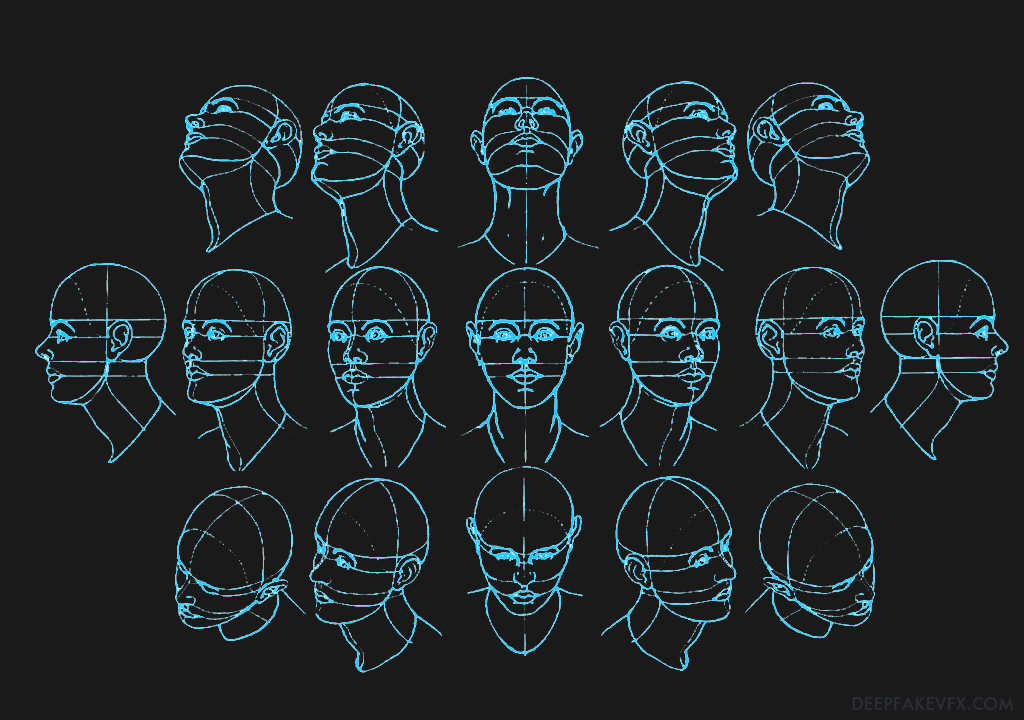
\includegraphics[width=0.5\textwidth]{Bilder/DFL/Human_Head_Angles_Diagram}
    \caption{Head Angles Diagram}
    \label{fig:head-angles-diagram}
\end{figure}

Ein Trainingsdatensatz sollte mehrere Hundert Bilder umfassen.
Je nach Resolution des trainierten Models sollten die Zahlen sogar in die Tausende gehen.\\[0.5cm]

Für den exemplarischen Deepfake dieser Arbeit, werden das mitgelieferte Standardvideo von \gls{rdj} als \texttt{Source} und das Interview von Prof. Dr. Harald Rieger und Prof. Volker Knoblauch als \texttt{Destination} verwendet.

\subsection{Pretraining}\label{subsec:pretraining}
Aus Gründen die in \ref{subsubsec:pretraining} beschrieben sind, wird ein Modell vortrainiert.
\gls{dfl} liefert bereits einen Datensatz zum Vortrainieren mit.
Das Pretraining kann also ohne weitere Vorbereitung beginnen.
\subsubsection*{Pretrain XSeg}
\begin{lstlisting}[label={lst:xseg-pretraining},numbers=none]
    5.XSeg) train.bat
\end{lstlisting}
Öffnet die Konsole für die Konfiguration.
\begin{itemize}
    \item \textbf{Face type:} Bestimmt wie viel von einem Gesicht ersetzt werden soll. Z.B. das Gesicht mit oder ohne Stirn usw.
    \item \textbf{Batch\_size:} Je höher die Batch size, desto größer die Hardwareanforderungen und desto besser die Ergebnisse
    \item \textbf{Enable pretraining mode:} Selbsterklärend
\end{itemize}
Nach einem Test ob die Hardware ausreichend für die Konfiguration ist, startet das Training (Abbildung \ref{fig:xseg-pretrain}).
Das Pretraining für XSeg kommt schon mit einigen Zehntausend Iterationen aus.
\begin{figure}
    \center
    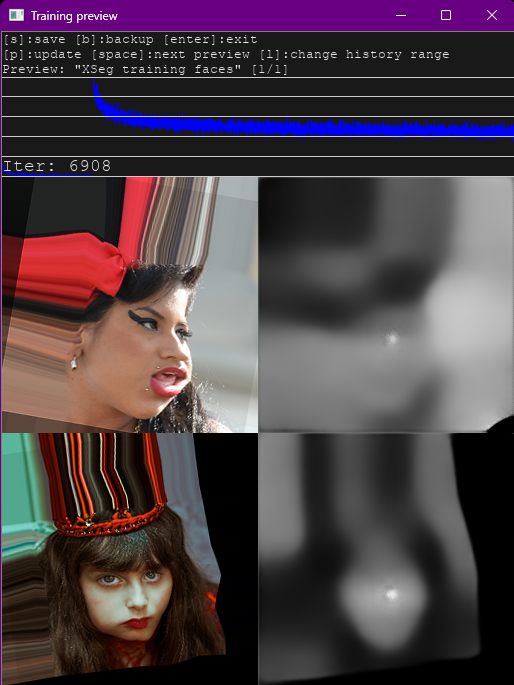
\includegraphics[width=0.7\textwidth]{Bilder/DFL/XSegEditor-3-pretrain}
    \caption{XSeg Pretraining im \textit{head} Modus}
    \label{fig:xseg-pretrain}
\end{figure}

\subsubsection*{Pretrain SAEHD}
\begin{lstlisting}[label={lst:saehd-pretraining},numbers=none]
    6) train SAEHD.bat
\end{lstlisting}
Dies öffnet die Konsole um ein neues Modell zu konfigurieren.
Für das Pretraining können alle Einstellungen, außer wenige Ausnahmen, auf Standard gelassen werden.
Geändert werden sollten die Folgenden:
\begin{itemize}
    \item \textbf{Autobackup every N hour:} Selbsterklärend
    \item \textbf{Target iteration:} Sinnvolle Werte für Pretraining sind 500 Tausend bis 1 Million
    \item \textbf{Resolution:} Je höher der Wert, desto hochaufgelöster das Ergebnis. Für \texttt{face} und \texttt{whole-face} sind $128$ ausreichend. Für \texttt{head} mindestens $224$. Für das bestmögliche Ergebnis so hoch setzten wie die Hardware mithalten kann.
    \item \textbf{Face type:} Bestimmt wie viel von einem Gesicht ersetzt werden soll. Z.B. das Gesicht mit oder ohne Stirn usw.
    \item \textbf{Batch\_size:} Analog zu Resolution. Nachdem sich für eine Resolution entschieden wurde, so hoch setzten bis die Hardware ausgelastet ist.
    \item \textbf{Enable pretraining mode:} Selbsterklärend
\end{itemize}
Nun wird ebenfalls die Hardware getestet und das Training gestartet (Abbildung \ref{fig:saehd-pretrain}).
\begin{figure}
    \center
    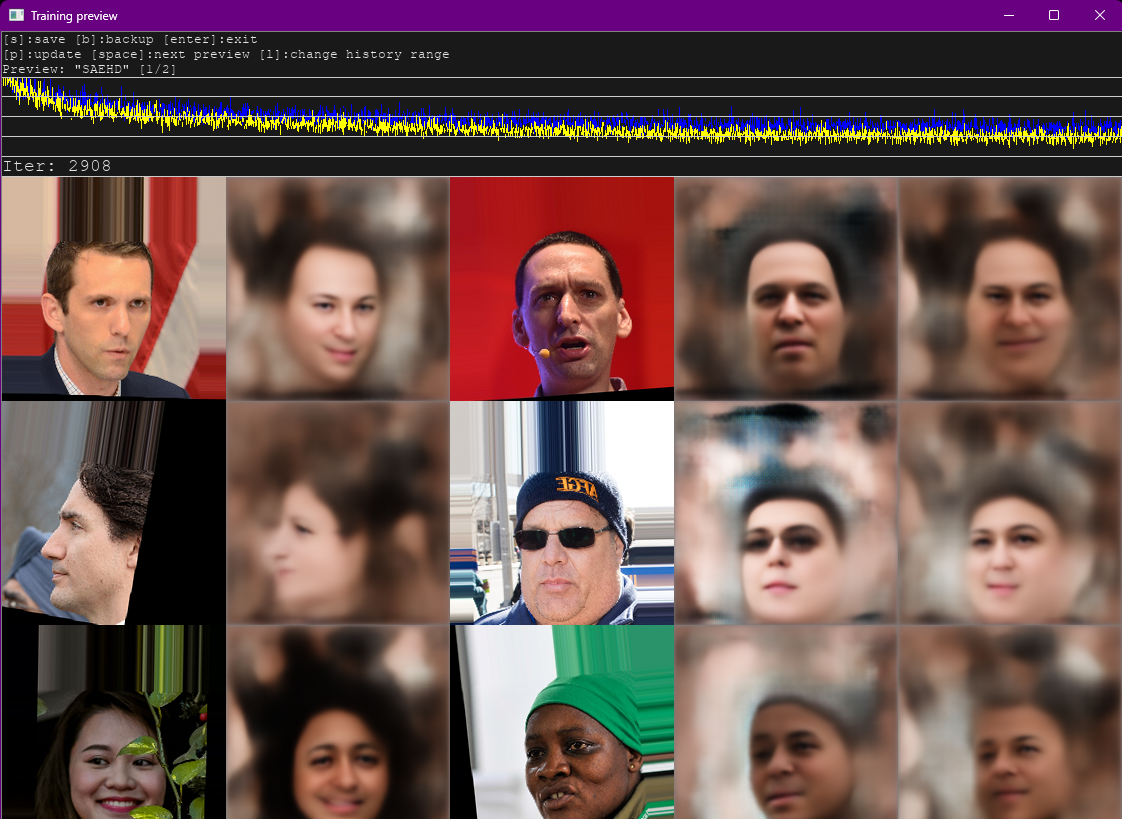
\includegraphics[width=0.7\textwidth]{Bilder/DFL/saehd-pretrain-head}
    \caption{SAEHD Pretraining mit 224 Resolution im \textit{head} Modus}
    \label{fig:saehd-pretrain}
\end{figure}